\documentclass{scrartcl}
\usepackage[margin=3cm]{geometry}
\usepackage{amsmath}
\usepackage{amssymb}
\usepackage{amsthm}
\usepackage{blindtext}
\usepackage{datetime}
\usepackage{fontspec}
\usepackage{float}
\usepackage{graphicx}
\usepackage{kotex}
\usepackage[lighttt]{lmodern}
\usepackage{listings}
\usepackage{mathrsfs}
\usepackage{mathtools}
\usepackage{pgf,tikz,pgfplots}
\usepackage{pdfpages}
\usepackage{tabularx}

\pgfplotsset{compat=1.15}
\usetikzlibrary{arrows}
\newtheorem{theorem}{Theorem}

\lstset{
  numbers=none, frame=single, showspaces=false,
  showstringspaces=false, showtabs=false, breaklines=true, showlines=true,
  breakatwhitespace=true, basicstyle=\ttfamily, keywordstyle=\bfseries, basewidth=0.5em
}

\setmainhangulfont{Noto Serif CJK KR}[
  UprightFont=* Light, BoldFont=* Bold,
  Script=Hangul, Language=Korean, AutoFakeSlant,
]
\setsanshangulfont{Noto Sans CJK KR}[
  UprightFont=* DemiLight, BoldFont=* Medium,
  Script=Hangul, Language=Korean
]
\setmathhangulfont{Noto Sans CJK KR}[
  SizeFeatures={
    {Size=-6,  Font=* Medium},
    {Size=6-9, Font=*},
    {Size=9-,  Font=* DemiLight},
  },
  Script=Hangul, Language=Korean
]
\title{CSED311: Lab 3 (due Apr. 16)}
\author{김태연(20220140), 손량(20220323)}
\date{Last compiled on: \today, \currenttime}

\newcommand{\un}[1]{\ensuremath{\ \mathrm{#1}}}

\begin{document}
\maketitle

\section{Introduction}
RISC-V architecture를 바탕으로 구성된 Multicycle CPU를 구현한다.

\section{Design}
이번에 구현한 RISC-V Multicycle CPU는 다음과 같은 주요 기능을 가진 Submodule로 나누었으며, 생성된 값들을 선택하기 위해
추가적으로 Multiplexer를 구현하여 사용했다. 기존 Single-cycle CPU에서 추가로 제작한 Adder는 ALU에서 재사용되었기 때문에
더 이상 필요로 하지 않는다.

\subsection{Program Counter}
기존 Single-cycle CPU에서는 Program Counter가 Clock signal에 Synchronous하게 무조건적으로 반영되었다.
Multicycle CPU의 구현에서는 Clock signal에 Synchronous하면서도, 추가적인 Control signal인
\texttt{pc\_write} 및 \texttt{pc\_commit} Signal에 따라 동작한다. \texttt{pc\_write} Signal은
Jump instruction 혹은 Branch instruction 여부 및 ALU의 Branch condition에 따라 활성화되며,
\texttt{pc\_commit}는 Multicycle CPU의 Instruction 별 Stage에서 Program counter가 갱신되어야 할
시점에 활성화되도록 Control unit에서 구현하였다.

\subsection{Memory}
기존 Single-cycle CPU에서는 Instruction Memory와 Data Memory가 별도로 분리되어 있었지만, Multicycle CPU에서는
해당 구분 없이 하나의 통합된 32bit\times16384 = 64KiB의 메모리를 사용한다. Memory 접근 이후 값을 전달할 때, Memory
Data Register (\texttt{inst\_reg}) 및 Instruction Register(\texttt{mem\_data\_reg})에 전달하게 된다.

\subsubsection{Memory Data Register}
Skeleton Code에서 주어진 \texttt{MDR}에 Clock signal과 Synchronous하게 Memory 모듈의 \texttt{dout}으로부터
나온 데이터를 저장한다. Clock signal에 따라 항상 값을 쓸 수 있다.
Memory Data Register의 값은 다음과 같은 용도로 사용된다.
\begin{itemize}
  \item Register File에 값을 Write back 하기 위한 값을 제공한다.
\end{itemize}

\subsubsection{Instruction Register}
Skeleton Code에서 주어진 \texttt{IR}에 Clock signal과 Synchronous하게 Memory 모듈의 \texttt{dout}으로부터
나온 데이터를 저장한다. Memory Data Register와 구현이 유사하나, Instruction Register는 Clock에 Synchronous하면서
Control Unit의 \texttt{ctrl\_unit\_inst\_reg\_write} Signal이 Enable 되었을 때만 작성될 수 있다.
Instruction Register의 값은 다음과 같은 용도로 사용된다.
\begin{itemize}
  \item Register File에 접근하기 위한 \texttt{rs1}, \texttt{rs2}, \texttt{rd} 와 같은 Register 정보를 제공한다.
  \item Immediate Generator에서 상수를 생성하는데 사용된다.
  \item Control Unit 및 ALU Control Unit에서 Control signal을 생성하기 위한 정보를 제공한다.
  \item Ecall Unit에서 \texttt{ecall}을 판단하기 위해 사용된다.
\end{itemize}

\subsection{Register File}
Single-cycle CPU와 마찬가지로 Clock signal에 Synchronous하게 Register value를 입력받고 갱신한다.
\subsubsection{Operand Register -- \texttt{A}, \texttt{B}}
Register file의 출력을 Clock signal에 맞추어 저장하는 temporaries이며, 입력된 다음 Cycle에 ALU의 입력으로
(각각의 Multiplexer에서 선택되었을 경우) 그 값을 전달한다.

\subsection{ALU}
Single-cycle CPU와 마찬가지로 \texttt{alu\_op}에 따라 연산을 결정하고, Clock signal과 Asynchronous하게
Register value 혹은 Immediate value로부터 값을 계산하여 출력한다. Branch condition의 경우는 Lab2에서 구현한
방식과 동일하게 LSB 1bit에 boolean 연산의 결과를 전달하도록 설계하였다.

\subsubsection{ALU Register -- \texttt{ALUOut}}
ALU의 출력을 Clock signal에 맞추어 \texttt{ALUOut}에 전달하며, (현재 Cycle의 ALU 연산 결과)와
(이전 Cycle의 ALU 연산 결과를 \texttt{ALUOut}에 저장한 값)중 적절한 값을 Register file에 Write back
하거나 Program counter을 갱신하는데 사용한다.

\subsection{Immediate Generator}
RV32I instruction 중 immediate value를 가지는 instruction의 타입이 존재하며, 각 타입 별 Immediate value가
생성되는 부분들 또한 다르다. Single-cycle CPU와 마찬가지의 구현으로, Clock signal과 Asynchronous하게
값을 계산하여 출력한다. 각 Instruction opcode의 type에 따라 생성해야 할 Immediate value를
immediate generator의 출력으로 전달한다.

\subsection{Control Unit}
어떤 Instruction type이던, LSB 7bit는 RV32I에서 opcode로 정의가 되어 있는 부분이다. Clock Signal에 Synchronous하게
Control Unit에서 현재 Instruction과 현재 State로부터 다음 Multicycle CPU Stage로 전환하였다.
이와 병렬적으로, \texttt{always @(*)}를 사용하여 각 CPU State 및 Instruction의 조합에서 CPU Control signal을
CPU Clock과 Asynchronous하게 생성하도록 설계하였다.

\subsection{Ecall Unit}
프로그램의 종료를 판별하기 위한 Ecall의 구조를 정의하였으며, Clock signal과 asynchronous하게 수행된다.


\section{State Design}
\subsection{State Design -- Stage}
Multicycle CPU를 구현하면서, Instruction이 각 Stage에 다음과 같은 작업을 수행하도록 분할하였다.

\subsubsection{R-type Register Arithmetic}
\begin{tabularx}{\textwidth}{ | c | X | }
  \hline
  \textbf{State} & \textbf{Action} \\ \hline
  \textbf{IF} & Instruction Fetch \newline \texttt{PC <- PC + 4} \\ \hline
  \textbf{ID} & Instruction Decode \newline \texttt{alu\_reg <- PC + imm} \\ \hline
  \textbf{EX} & \texttt{alu\_reg <- reg\_file[rs1] op reg\_file[rs2]} (for value) \\ \hline
  \textbf{MEM} & \textit{Pass} \\ \hline
  \textbf{WB} & Save \texttt{alu\_reg} to \texttt{reg\_file[rd]} \\
  \hline
\end{tabularx}

\subsubsection{I-type Immediate Arithmetic}
\begin{tabularx}{\textwidth}{ | c | X | }
  \hline
  \textbf{State} & \textbf{Action} \\ \hline
  \textbf{IF} & Instruction Fetch \newline \texttt{PC <- PC + 4} \\ \hline
  \textbf{ID} & Instruction Decode \newline \texttt{alu\_reg <- PC + imm} \\ \hline
  \textbf{EX} & \texttt{alu\_reg <- reg\_file[rs1] op imm} (for value) \\ \hline
  \textbf{MEM} & \textit{Pass} \\ \hline
  \textbf{WB} & Save \texttt{alu\_reg} to \texttt{reg\_file[rd]} \\
  \hline
\end{tabularx}

\subsubsection{I-type Load}
\begin{tabularx}{\textwidth}{ | c | X | }
  \hline
  \textbf{State} & \textbf{Action} \\ \hline
  \textbf{IF} & Instruction Fetch \newline \texttt{PC <- PC + 4} \\ \hline
  \textbf{ID} & Instruction Decode \newline \texttt{alu\_reg <- PC + imm} \\ \hline
  \textbf{EX} & \texttt{alu\_reg <- reg\_file[rs1] op imm} (for address) \\ \hline
  \textbf{MEM} & Save memory to \texttt{mem\_data\_reg} \\ \hline
  \textbf{WB} & Save \texttt{mem\_data\_reg} to \texttt{reg\_file[rd]} \\
  \hline
\end{tabularx}

\subsubsection{S-type Store}
\begin{tabularx}{\textwidth}{ | c | X | }
  \hline
  \textbf{State} & \textbf{Action} \\ \hline
  \textbf{IF} & Instruction Fetch \newline \texttt{PC <- PC + 4} \\ \hline
  \textbf{ID} & Instruction Decode \newline \texttt{alu\_reg <- PC + imm} \\ \hline
  \textbf{EX} & \texttt{alu\_reg <- reg[rs1] op imm} (for address) \\ \hline
  \textbf{MEM} & Save \texttt{memory[reg[rs2]] <- alu\_reg} \\ \hline
  \textbf{WB} & \textit{Pass} \\
  \hline
\end{tabularx}

\subsubsection{B-type Branch}
\begin{tabularx}{\textwidth}{ | c | X | }
  \hline
  \textbf{State} & \textbf{Action} \\ \hline
  \textbf{IF} & Instruction Fetch \newline \texttt{PC <- PC + 4} \\ \hline
  \textbf{ID} & Instruction Decode \newline \texttt{alu\_reg <- PC + imm} \\ \hline
  \textbf{EX} & \texttt{reg[rs1] op reg[rs2]} (for branch condition) \newline Update \texttt{pc} with condition \\ \hline
  \textbf{MEM} & \textit{Pass} \\ \hline
  \textbf{WB} & \textit{Pass} \\
  \hline
\end{tabularx}

\subsubsection{J-type \texttt{JAL}}
\begin{tabularx}{\textwidth}{ | c | X | }
  \hline
  \textbf{State} & \textbf{Action} \\ \hline
  \textbf{IF} & Instruction Fetch \newline \texttt{PC <- PC + 4} \\ \hline
  \textbf{ID} & Instruction Decode \newline \texttt{alu\_reg <- PC + imm} \newline \texttt{reg\_file[rd] <- pc + 4} \\ \hline
  \textbf{EX} & \texttt{pc <- alu\_reg} \\ \hline
  \textbf{MEM} & \textit{Pass} \\ \hline
  \textbf{WB} & \textit{Pass} \\
  \hline
\end{tabularx}

\subsubsection{J-type \texttt{JALR}}
\begin{tabularx}{\textwidth}{ | c | X | }
  \hline
  \textbf{State} & \textbf{Action} \\ \hline
  \textbf{IF} & Instruction Fetch \newline \texttt{PC <- PC + 4} \\ \hline
  \textbf{ID} & Instruction Decode \newline \texttt{alu\_reg <- PC + imm} \newline \texttt{reg\_file[rd] <- pc + 4} \\ \hline
  \textbf{EX} & \texttt{pc <- reg\_file[rs1] + imm} \\ \hline
  \textbf{MEM} & \textit{Pass} \\ \hline
  \textbf{WB} & \textit{Pass} \\
  \hline
\end{tabularx}

\subsection{State Design -- State Transition}
Multicycle CPU에서 특정 Instruction에 필요한 Stage만 수행하기 위한 State Transition을 작성하여 설계하였다.
아래 표에 특정 Instruction의 Stage 간 Transition을 나타내었으며, 해당 Transition은 \texttt{control\_unit.v}에서
\texttt{case(state)} 및 \texttt{next\_state}를 Instruction type별로 Setting하는 것을 확인할 수 있다.
\begin{center}
  \begin{tabular}{ | c | c | c | c | c | c | c | c |}
    \hline
    \textbf{Type} & \textbf{Instruction} & \textbf{IF} & \textbf{ID} & \textbf{EX} & \textbf{MEM} & \textbf{WB} \\ \hline
    R & Arithmetic & ID & EX & WB & - & IF \\ \hline
    I & Arithmetic & ID & EX & WB & - & IF \\ \hline
    I & Load & ID & EX & MEM & WB & IF \\ \hline
    S & Store & ID & EX & MEM & IF & - \\ \hline
    B & Branch & ID & EX & IF & - & - \\ \hline
    J & \texttt{JAL} & ID & EX & IF & - & - \\ \hline
    I & \texttt{JALR} & ID & EX & IF & - & - \\ \hline
  \end{tabular}
\end{center}

\subsection{State Design -- Control Signal}
이를 구현하기 위해, Control Unit에서는 각 Stage에 다음과 같은 Signal을 생성한다. \texttt{0} 혹은 \texttt{1}을 가지지 않는
Multiplexer의 select는 Selection의 Definition을 작성했다.
\begin{itemize}
  \item \texttt{ecall} 의 경우, 추가적으로 \texttt{ECALL} type instruction을 정의했으나 아래 테이블에는 추가하지 않았다.
  \item \texttt{2b'00} in \texttt{wb\_sel} and \texttt{op2\_sel} -- Enumeration을 가짐에도 \texttt{2b'00} 형태의
  입력을 가지는 경우는 Don't care term으로 사용된다.
  \item \texttt{4b'0000} in \texttt{alu\_op} -- 해당 Control unit에서 나오는 \texttt{alu\_op} signal은 직접 ALU에 들어가지 않고,
  ALU Control Unit을 거쳐 들어가게 된다. 이 때, ALU Control Unit의 \texttt{alu\_op\_from\_inst} Control signal이 Disable된 경우
  ALU Control Unit의 입력 signal을 ALU로 전파한다. 아래의 표에서 \texttt{4b'0000}의 경우에 해당하며, ALU는 Instruction으로부터 결정된 Operation을 수행한다.
\end{itemize}

\subsubsection{R-type Register Arithmetic}
\begin{tabularx}{\textwidth}{ | X | c | c | c | c | c | }
  \hline
  \textbf{Signal} & \textbf{IF} & \textbf{ID} & \textbf{EX} & \textbf{MEM} & \textbf{WB} \\ \hline
  \texttt{inst\_reg\_write} & 1 & 0 & 0 & - & 0 \\ \hline
  \texttt{data\_access} & 0 & 0 & 0 & - & 0 \\ \hline
  \texttt{mem\_read} & 1 & 0 & 0 & - & 0 \\ \hline
  \texttt{mem\_write} & 0 & 0 & 0 & - & 0 \\ \hline
  \texttt{op\_reg\_write} & 0 & 1 & 0 & - & 0 \\ \hline
  \texttt{op1\_regfile} & 0 & 0 & 1 & - & 0 \\ \hline
  \texttt{op2\_sel} & \texttt{OP2\_FOUR} & \texttt{OP2\_IMM} & \texttt{OP2\_REG} & - & 00 \\ \hline
  \texttt{alu\_reg\_write} & 0 & 1 & 1 & - & 0 \\ \hline
  \texttt{alu\_op\_from\_inst} & 0 & 0 & 1 & - & 0 \\ \hline
  \texttt{alu\_op} & \multicolumn{3}{c|}{\texttt{ALU\_ADD}} & - & 0000 \\ \hline
  \texttt{mem\_reg\_write} & 0 & 0 & 0 & - & 0 \\ \hline
  \texttt{regfile\_write} & 0 & 0 & 0 & - & 1 \\ \hline
  \texttt{wb\_sel} & 00 & 00 & 00 & - & \texttt{WB\_ALU\_REG} \\ \hline
  \texttt{pc\_write\_cond} & 0 & 0 & 0 & - & 0 \\ \hline
  \texttt{pc\_write} & 1 & 0 & 0 & - & 0 \\ \hline
  \texttt{pc\_commit} & 0 & 0 & 0 & - & 1 \\ \hline
  \texttt{pc\_from\_alu\_reg} & 0 & 0 & 0 & - & 0 \\ \hline
\end{tabularx}

\subsubsection{I-type Immediate Arithmetic}
\begin{tabularx}{\textwidth}{ | X | c | c | c | c | c | }
  \hline
  \textbf{Signal} & \textbf{IF} & \textbf{ID} & \textbf{EX} & \textbf{MEM} & \textbf{WB} \\ \hline
  \texttt{inst\_reg\_write} & 1 & 0 & 0 & - & 0 \\ \hline
  \texttt{data\_access} & 0 & 0 & 0 & - & 0 \\ \hline
  \texttt{mem\_read} & 1 & 0 & 0 & - & 0 \\ \hline
  \texttt{mem\_write} & 0 & 0 & 0 & - & 0 \\ \hline
  \texttt{op\_reg\_write} & 0 & 1 & 0 & - & 0 \\ \hline
  \texttt{op1\_regfile} & 0 & 0 & 1 & - & 0 \\ \hline
  \texttt{op2\_sel} & \texttt{OP2\_FOUR} & \texttt{OP2\_IMM} & \texttt{OP2\_REG} & - & 00 \\ \hline
  \texttt{alu\_reg\_write} & 0 & 1 & 1 & - & 0 \\ \hline
  \texttt{alu\_op\_from\_inst} & 0 & 0 & 1 & - & 0 \\ \hline
  \texttt{alu\_op} & \multicolumn{3}{c|}{\texttt{ALU\_ADD}} & - & 0000 \\ \hline
  \texttt{mem\_reg\_write} & 0 & 0 & 0 & - & 0 \\ \hline
  \texttt{regfile\_write} & 0 & 0 & 0 & - & 1 \\ \hline
  \texttt{wb\_sel} & 00 & 00 & 00 & - & \texttt{WB\_ALU\_REG} \\ \hline
  \texttt{pc\_write\_cond} & 0 & 0 & 0 & - & 0 \\ \hline
  \texttt{pc\_write} & 1 & 0 & 0 & - & 0 \\ \hline
  \texttt{pc\_commit} & 0 & 0 & 0 & - & 1 \\ \hline
  \texttt{pc\_from\_alu\_reg} & 0 & 0 & 0 & - & 0 \\ \hline
\end{tabularx}

\subsubsection{I-type Load}
\begin{tabularx}{\textwidth}{ | X | c | c | c | c | c | }
  \hline
  \textbf{Signal} & \textbf{IF} & \textbf{ID} & \textbf{EX} & \textbf{MEM} & \textbf{WB} \\ \hline
  \texttt{inst\_reg\_write} & 1 & 0 & 0 & 0 & 0 \\ \hline
  \texttt{data\_access} & 0 & 0 & 0 & 1 & 0 \\ \hline
  \texttt{mem\_read} & 1 & 0 & 0 & 1 & 0 \\ \hline
  \texttt{mem\_write} & 0 & 0 & 0 & 0 & 0 \\ \hline
  \texttt{op\_reg\_write} & 0 & 1 & 0 & 0 & 0 \\ \hline
  \texttt{op1\_regfile} & 0 & 0 & 1 & 0 & 0 \\ \hline
  \texttt{op2\_sel} & \texttt{OP2\_FOUR} & \texttt{OP2\_IMM} & \texttt{OP2\_IMM} & 00 & 00 \\ \hline
  \texttt{alu\_reg\_write} & 0 & 1 & 1 & 0 & 0 \\ \hline
  \texttt{alu\_op\_from\_inst} & 0 & 0 & 0 & 0 & 0 \\ \hline
  \texttt{alu\_op} & \multicolumn{3}{c|}{\texttt{ALU\_ADD}} & 0000 & 0000 \\ \hline
  \texttt{mem\_reg\_write} & 0 & 0 & 0 & 1 & 0 \\ \hline
  \texttt{regfile\_write} & 0 & 0 & 0 & 0 & 1 \\ \hline
  \texttt{wb\_sel} & 00 & 00 & 00 & 00 & \texttt{WB\_MEM} \\ \hline
  \texttt{pc\_write\_cond} & 0 & 0 & 0 & 0 & 0 \\ \hline
  \texttt{pc\_write} & 1 & 0 & 0 & 0 & 0 \\ \hline
  \texttt{pc\_commit} & 0 & 0 & 0 & 0 & 1 \\ \hline
  \texttt{pc\_from\_alu\_reg} & 0 & 0 & 0 & 0 & 0 \\ \hline
\end{tabularx}

\subsubsection{S-type Store}
\begin{tabularx}{\textwidth}{ | X | c | c | c | c | c | }
  \hline
  \textbf{Signal} & \textbf{IF} & \textbf{ID} & \textbf{EX} & \textbf{MEM} & \textbf{WB} \\ \hline
  \texttt{inst\_reg\_write} & 1 & 0 & 0 & 0 & - \\ \hline
  \texttt{data\_access} & 0 & 0 & 0 & 1 & - \\ \hline
  \texttt{mem\_read} & 1 & 0 & 0 & 0 & - \\ \hline
  \texttt{mem\_write} & 0 & 0 & 0 & 1 & - \\ \hline
  \texttt{op\_reg\_write} & 0 & 1 & 0 & 0 & - \\ \hline
  \texttt{op1\_regfile} & 0 & 0 & 1 & 0 & - \\ \hline
  \texttt{op2\_sel} & \texttt{OP2\_FOUR} & \texttt{OP2\_IMM} & \texttt{OP2\_IMM} & 00 & - \\ \hline
  \texttt{alu\_reg\_write} & 0 & 1 & 1 & 0 & - \\ \hline
  \texttt{alu\_op\_from\_inst} & 0 & 0 & 0 & 0 & - \\ \hline
  \texttt{alu\_op} & \multicolumn{3}{c|}{\texttt{ALU\_ADD}} & 0000 & - \\ \hline
  \texttt{mem\_reg\_write} & 0 & 0 & 0 & 0 & - \\ \hline
  \texttt{regfile\_write} & 0 & 0 & 0 & 0 & - \\ \hline
  \texttt{wb\_sel} & 00 & 00 & 00 & 00 & - \\ \hline
  \texttt{pc\_write\_cond} & 0 & 0 & 0 & 0 & - \\ \hline
  \texttt{pc\_write} & 1 & 0 & 0 & 0 & - \\ \hline
  \texttt{pc\_commit} & 0 & 0 & 1 & 0 & - \\ \hline
  \texttt{pc\_from\_alu\_reg} & 0 & 0 & 0 & 0 & - \\ \hline
\end{tabularx}

\subsubsection{B-type Branch}
\begin{tabularx}{\textwidth}{ | X | c | c | c | c | c | }
  \hline
  \textbf{Signal} & \textbf{IF} & \textbf{ID} & \textbf{EX} & \textbf{MEM} & \textbf{WB} \\ \hline
  \texttt{inst\_reg\_write} & 1 & 0 & 0 & - & - \\ \hline
  \texttt{data\_access} & 0 & 0 & 0 & - & - \\ \hline
  \texttt{mem\_read} & 1 & 0 & 0 & - & - \\ \hline
  \texttt{mem\_write} & 0 & 0 & 0 & - & - \\ \hline
  \texttt{op\_reg\_write} & 0 & 1 & 0 & - & - \\ \hline
  \texttt{op1\_regfile} & 0 & 0 & 1 & - & - \\ \hline
  \texttt{op2\_sel} & \texttt{OP2\_FOUR} & \texttt{OP2\_IMM} & \texttt{OP2\_REG} & - & - \\ \hline
  \texttt{alu\_reg\_write} & 0 & 1 & 0 & - & - \\ \hline
  \texttt{alu\_op\_from\_inst} & 0 & 0 & 1 & - & - \\ \hline
  \texttt{alu\_op} & \multicolumn{3}{c|}{\texttt{ALU\_ADD}} & - & - \\ \hline
  \texttt{mem\_reg\_write} & 0 & 0 & 0 & - & - \\ \hline
  \texttt{regfile\_write} & 0 & 0 & 0 & - & - \\ \hline
  \texttt{wb\_sel} & 00 & 00 & 00 & - & - \\ \hline
  \texttt{pc\_write\_cond} & 0 & 0 & 1 & - & - \\ \hline
  \texttt{pc\_write} & 1 & 0 & 0 & - & - \\ \hline
  \texttt{pc\_commit} & 0 & 0 & 1 & - & - \\ \hline
  \texttt{pc\_from\_alu\_reg} & 0 & 0 & 1 & - & - \\ \hline
\end{tabularx}

\subsubsection{J-type \texttt{JAL}}
\begin{tabularx}{\textwidth}{ | X | c | c | c | c | c | }
  \hline
  \textbf{Signal} & \textbf{IF} & \textbf{ID} & \textbf{EX} & \textbf{MEM} & \textbf{WB} \\ \hline
  \texttt{inst\_reg\_write} & 1 & 0 & 0 & - & - \\ \hline
  \texttt{data\_access} & 0 & 0 & 0 & - & - \\ \hline
  \texttt{mem\_read} & 1 & 0 & 0 & - & - \\ \hline
  \texttt{mem\_write} & 0 & 0 & 0 & - & - \\ \hline
  \texttt{op\_reg\_write} & 0 & 1 & 0 & - & - \\ \hline
  \texttt{op1\_regfile} & 0 & 0 & 0 & - & - \\ \hline
  \texttt{op2\_sel} & \texttt{OP2\_FOUR} & \texttt{OP2\_IMM} & \texttt{OP2\_IMM} & - & - \\ \hline
  \texttt{alu\_reg\_write} & 0 & 1 & 0 & - & - \\ \hline
  \texttt{alu\_op\_from\_inst} & 0 & 0 & 0 & - & - \\ \hline
  \texttt{alu\_op} & \multicolumn{3}{c|}{\texttt{ALU\_ADD}} & - & - \\ \hline
  \texttt{mem\_reg\_write} & 0 & 0 & 0 & - & - \\ \hline
  \texttt{regfile\_write} & 0 & 1 & 0 & - & - \\ \hline
  \texttt{wb\_sel} & 00 & \texttt{WB\_PC\_NEXT\_TEMP} & 00 & - & - \\ \hline
  \texttt{pc\_write\_cond} & 0 & 0 & 0 & - & - \\ \hline
  \texttt{pc\_write} & 1 & 0 & 1 & - & - \\ \hline
  \texttt{pc\_commit} & 0 & 0 & 1 & - & - \\ \hline
  \texttt{pc\_from\_alu\_reg} & 0 & 0 & 1 & - & - \\ \hline
\end{tabularx}

\subsubsection{I-type \texttt{JALR}}
\begin{tabularx}{\textwidth}{ | X | c | c | c | c | c | }
  \hline
  \textbf{Signal} & \textbf{IF} & \textbf{ID} & \textbf{EX} & \textbf{MEM} & \textbf{WB} \\ \hline
  \texttt{inst\_reg\_write} & 1 & 0 & 0 & - & - \\ \hline
  \texttt{data\_access} & 0 & 0 & 0 & - & - \\ \hline
  \texttt{mem\_read} & 1 & 0 & 0 & - & - \\ \hline
  \texttt{mem\_write} & 0 & 0 & 0 & - & - \\ \hline
  \texttt{op\_reg\_write} & 0 & 1 & 0 & - & - \\ \hline
  \texttt{op1\_regfile} & 0 & 0 & 1 & - & - \\ \hline
  \texttt{op2\_sel} & \texttt{OP2\_FOUR} & \texttt{OP2\_IMM} & \texttt{OP2\_IMM} & - & - \\ \hline
  \texttt{alu\_reg\_write} & 0 & 1 & 0 & - & - \\ \hline
  \texttt{alu\_op\_from\_inst} & 0 & 0 & 0 & - & - \\ \hline
  \texttt{alu\_op} & \multicolumn{3}{c|}{\texttt{ALU\_ADD}} & - & - \\ \hline
  \texttt{mem\_reg\_write} & 0 & 0 & 0 & - & - \\ \hline
  \texttt{regfile\_write} & 0 & 1 & 0 & - & - \\ \hline
  \texttt{wb\_sel} & 00 & \texttt{WB\_PC\_NEXT\_TEMP} & 00 & - & - \\ \hline
  \texttt{pc\_write\_cond} & 0 & 0 & 0 & - & - \\ \hline
  \texttt{pc\_write} & 1 & 0 & 1 & - & - \\ \hline
  \texttt{pc\_commit} & 0 & 0 & 1 & - & - \\ \hline
  \texttt{pc\_from\_alu\_reg} & 0 & 0 & 0 & - & - \\ \hline
\end{tabularx}

\section{Implementation}
각 베릴로그 파일에 대한 세부 설명은 다음과 같다.

\subsection{\texttt{top.v} -- Top module}
\texttt{cpu.v}에서 구현한 \texttt{cpu} 모듈을 사용하여 Multi cycle CPU를 구현하였다.

\subsection{\texttt{cpu.v} -- 내부 Module을 연결하여 Multicycle CPU 구성}
\texttt{cpu.v}는 다음과 같은 submodule을 연결하여 구성하였다.
\begin{itemize}
\item \texttt{pc pc\_mod} -- Program counter을 구현하였다.
\item \texttt{RegisterFile reg\_file} -- Register file으로, 값의 Read는 Asynchronous하게,  Write는 control signal에 따라 Synchronous하게 작성할 수 있다.
\item \texttt{operand\_register op\_reg} -- Register file의 Output을 ALU로 전달하기 위한 레지스터인 \texttt{A} 와 \texttt{B}를 관리하며, Clock cycle에 Synchronous하게 값을 쓸 수 있다.
\item \texttt{mux32bit\_4x1 reg\_file\_write\_data\_mux} -- Register file에 들어갈 수 있는 값을 선택하기 위한 Multiplexer를 구현하였다.
\item \texttt{Memory memory} -- Data memory와 Instruction memory가 통합된 하나의 Memory를 사용하고 있으며, Read 및 Write 모두 Clock signal에 Synchronous하게 접근한다.
\item \texttt{memory\_data\_register mem\_data\_reg} -- Memory에서 가져온 Data를 임시로 저장하기 위한 레지스터인 \texttt{MDR}에 Clock signal에 Synchronous하게 값을 작성한다.
\item \texttt{mux32bit\_2x1 memory\_addr\_mux} -- 통합된 Memory에서, Data 영역에 접근할 지 Instruction 영역에 접근할 지 선택하도록 Multiplexer를 구현하였다.
\item \texttt{control\_unit ctrl\_unit} -- CPU의 Microsequence를 Instruction에 따라 관리하며, Microsequence의 진행과 각 Stage 별 Control signal을 조절한다.
\item \texttt{instruction\_register inst\_reg} -- Memory에서 가져온 Instruction을 임시로 저장하기 위한 레지스터인 \texttt{IR}에 Clock signal에 Synchronous하게 작성한다.
\item \texttt{ecall\_unit ec\_unit} -- \texttt{ecall}을 처리하기 위한 모듈을 구현하였다.
\item \texttt{immediate\_generator imm\_gen} -- 각 Instruction type에 해당하는 Immediate value를 생성한다.
\item \texttt{alu\_control\_unit alu\_ctrl\_unit} -- Instruction으로부터 ALU의 Opcode를 획득한다.
\item \texttt{alu alu\_mod} -- ALU를 구현하였다.
\item \texttt{alu\_register alu\_reg} -- ALU의 출력으로 \texttt{ALUOut} 레지스터에 Clock signal에 Synchronous하게 값을 작성한다.
\item \texttt{mux32bit\_2x1 alu\_in\_1\_mux} -- ALU의 \texttt{in\_1} 포트의 가능한 2개의 입력 중 적절한 입력을 선택한다.
\item \texttt{mux32bit\_4x1 alu\_in\_2\_mux} -- ALU의 \texttt{in\_2} 포트의 가능한 3개의 입력 중 적절한 입력을 선택한다.
\item \texttt{mux32bit\_2x1 pc\_source\_mux} -- 다음 Program counter의 값이 될 수 있는 입력 2개의 입력 중 적절한 입력을 선택한다.
\end{itemize}

\subsection{\texttt{control\_unit.v} -- 마이크로컨트롤러 구현}
각 Instruction type과 State에 따라, 다음과 같은 Control signal을 생성한다. Instruction 별 해당 Signal의 생성 시기는 앞에서 설명하였다.
\begin{itemize}
  \item \texttt{inst\_reg\_write} -- Instruction Register \texttt{IR}에 Memory unit의 출력을 Write하기 위한 Control signal이다.
  \item \texttt{data\_access} -- Memory에 Access하기 위해 Data address 혹은 Instruction address를 제공받는 Multiplexer의 Selection이다.
  \item \texttt{mem\_read} -- Memory로부터 값을 Read할 때 활성화되는 Control signal이다.
  \item \texttt{mem\_write} -- Memory에 값을 Write할 때 활성화되는 Control signal이다. 
  \item \texttt{op\_reg\_write} -- Register file의 출력에 있는 temporal register인 \texttt{A}, \texttt{B}에 Write하기 위한 Control signal이다.
  \item \texttt{op1\_regfile} -- ALU의 \texttt{op1} 입력으로 (현재 Program counter) / (\texttt{A})를 선택하는 Multiplexer의 Selection이다.
  \item \texttt{op2\_sel} -- ALU의 \texttt{op2} 입력으로 (\texttt{B}) / (\texttt{4}) / (Immediate generator output)을 선택하는 Multiplexer의 Selection이다.
  \item \texttt{is\_ecall} -- 현재 Instruction이 \texttt{ecall}인 경우 활성화되는 Control signal이다.
  \item \texttt{alu\_reg\_write} -- ALU result를 \texttt{ALUOut}에 Write하기 위한 Control signal이다.
  \item \texttt{alu\_op\_from\_inst} -- ALU Control Unit이 Instruction으로부터 ALU Operation을 결정하도록 하는 Control signal이다.
  \item \texttt{alu\_op} -- ALU가 수행할 Operation에 대한 코드이다. (\texttt{alu\_def.v} 참조)
  \item \texttt{mem\_reg\_write} -- Data Register \texttt{MDR}에 Memory unit의 출력을 Write하기 위한 Control signal을 구상하였으나, 해당 레지스터에는 조건 없이 Clock signal에 Synchronous하게 값을 작성한다.
  \item \texttt{regfile\_write} -- Register file에 값을 Write하기 위한 Control signal이다.
  \item \texttt{wb\_sel} -- Register file에 Write back될 값으로 (\texttt{ALUOut}) / (\texttt{MDR}) / (\texttt{PC + 4})를 선택하는 Multiplexer의 Selection이다.
  \item \texttt{pc\_write\_cond} -- Program counter를 업데이트하기 위한 Branch instruction에 활성화되는 입력으로, ALU의 result에 따라 Branch taken / Branch not taken을 판단한다.
  \item \texttt{pc\_write} -- \texttt{JAL} 및 \texttt{JALR} 의 Jump instruction을 통한 갱신 및 \texttt{PC + 4}로 갱신하는 Stage에서 활성화되는 Control signal이다.
  \item \texttt{pc\_commit} -- 다음 Program counter의 실제 업데이트를 진행하기 위한 Control signal이다.
  \item \texttt{pc\_from\_alu\_reg} -- Program counter의 Source로 (현재 ALU의 Result) / (\texttt{ALUOut})를 선택하는 Multiplexer의 Selection이다.
\end{itemize}
\subsubsection{\texttt{control\_unit\_def.v} -- 마이크로컨트롤러 상수 정의}
다음과 같은 종류들의 상수가 정의되어 있다.
\begin{itemize}
  \item \texttt{CTRL\_OP2\_xxx} -- ALU의 \texttt{in\_2} 입력을 결정하기 위한 4x1 MUX의 Selection 상수이다.
  \item \texttt{CTRL\_xx\_STAGE} -- Multicycle CPU의 각 Stage를 내부적으로 나타내기 위한 상수이다.
  \item \texttt{CTRL\_WB\_xxx} -- Register file의 Write back을 진행할 때, 4x1 MUX의 Selection 상수이다.
\end{itemize}

\subsection{\texttt{pc.v} -- Program counter 구현}
Clock signal에 Synchronous하게 작동하며, 입력으로 들어온 현재의 Program counter,
혹은 ALU의 연산 결과로부터 Program counter의 값을 갱신한다.
\texttt{pc} module은 다음과 같은 2개의 Control unit의 Signal에 따라 작동한다.
\begin{itemize}
  \item \texttt{pc\_write} -- 모든 Instruction Fetch Stage와 \texttt{JAL} 및 \texttt{JALR}에서 Program counter 값의 전달 및 저장을 위한 신호이다.
  \item \texttt{pc\_commit} -- 현재 Program counter의 값을 갱신하기 위한 신호이다.
\end{itemize}
해당 \texttt{pc} module은 2개의 출력을 가지며, 다음과 같다.
\begin{itemize}
  \item \texttt{current\_pc} -- 현재 Program counter의 값을 출력한다.
  \item \texttt{next\_temp\_pc} -- \texttt{JAL} 및 \texttt{JALR}에서 Program counter을 레지스터 파일에 직접 전달하기 위해 추가적인 Wire를 구성하였다.
\end{itemize}
두 개의 독립적인 신호를 입력받아 Program counter를 갱신함으로써, \texttt{JAL} 및 \texttt{JALR} instruction에서 사용되는 Cycle의 수를 줄일 수 있었다.
\texttt{pc\_write}을 통해 \texttt{pc\_next\_temp\_pc}로 다음 Program counter를 미리 계산하여, Register file의 입력으로 미리 계산된 Program counter를
선택하여 Write back을 진행할 수 있다. 미리 Register file에 값을 Write back 하고, 해당 값을 \texttt{pc\_commit}을 사용하여 Program counter에 반영한다.

\subsection{\texttt{Memory.v} -- 통합된 Memory 구현}
Single-cycle CPU와 다르게, Multicycle CPU에서는 Instruction memory 및 Data memory가 통합된 형태로 사용되고 있다.
Instruction 영역 혹은 Data 영역으로의 접근은 \texttt{addr}에 연결된 Multiplexer에서 선택하여 접근 가능하다.
Clock signal에 Synchronous하게 \texttt{mem\_read}, \texttt{mem\_write}의 신호가 주어졌을 때 각각 읽고 쓰기가 가능하다.
Memory의 출력은 \texttt{memory\_dout}을 통해 전달되며, 이는 아래의 \texttt{mem\_data\_reg} 과 \texttt{inst\_reg} 와 연결되어
값을 Clock signal에 Synchronous하게 전달한다.

\subsubsection{\texttt{memory\_data\_register.v} -- Data memory register 구현}
Memory unit에서 memory를 읽을 때 마다 \texttt{memory\_dout}으로 전달되고, \texttt{mem\_data\_reg}가 Clock signal에
Synchronous하게 \texttt{MDR}에 값을 전달한다.

\subsubsection{\texttt{instruction\_register.v} -- Instruction memory register 구현}
Memory unit에서 memory를 읽을 때 \texttt{memory\_dout}으로 값이 전달되고, Instruction 영역을 읽는 경우엔 \texttt{inst\_reg}의
\texttt{ir\_write}에 연결된 Control signal이 enable되어 Clock signal에 Synchronous하게 \texttt{IR}으로 Instruction을 전달한다.

\subsection{\texttt{RegisterFile.v} -- Register File 구현}
Single-cycle CPU와 동일한 구현 형태를 가지고 있다. Clock signal에 Synchronous하게 값을 작성할 수 있으며,
Multicycle CPU에서는 Write Back stage에서 작성되도록 Control signal을 설계하였다.
Hard-wired zero Register인 \texttt{reg\_file[0]} 에 작성 시 값이 변조되지 않도록 추가적인 조건을 추가하였다.
\texttt{x17} Register는 \texttt{ecall} 처리 후 \texttt{is\_halted}을 설정하는데 사용되게 되며, 이를 위해
추가적으로 해당 \texttt{x17} 레지스터만을 출력하는 wire를 가지고 있다.

\subsubsection{\texttt{operand\_register.v} -- Operand temporaries 구현}
Register file에서 얻은 Register value는 Skeleton code에서 주어진 temporary register인 \texttt{A}와 \texttt{B}으로
값이 전달된다. Clock signal에 Synchronous하게 값을 전달하게 되며, \texttt{A} 및 \texttt{B} 는 ALU의 입력을
결정하는 Multiplexer와 연결되어 Control signal에 따라 ALU의 피연산자가 될 수 있다.

\subsection{\texttt{immediate\_generator.v} -- Immediate generator 구현}
Single-cycle CPU에서 사용한 Immediate generator와 구조가 동일하다.
Instruction이 inst로 주어질 때 \texttt{opcode}, \texttt{func3} 값을 통해 immediate value를 생성하여
\texttt{imm}으로 출력하도록 구현하였다. 해당 동작은 Clock signal에 Asynchronous하게 작동한다.

\subsection{\texttt{alu.v} -- ALU 동작 구현}
Single-cycle CPU에서 사용한 ALU와 구조가 동일하며, Clock signal에 Asynchronous하게 동작하도록 구현하였다.
연산을 선택하기 위한 \texttt{alu\_op}에 따라 두 개의 32bit 입력에 해당하는 연산 결과를 \texttt{alu\_result} 에 반환한다.
산술 연산의 경우 32bit를 모두 사용하여 결과 값을 전달하였으며, 논리 연산의 경우 LSB 1bit에 해당 논리 연산의 결과를 반환하였다.
\subsubsection{\texttt{alu\_def.v} -- ALU 구성을 위한 상수 정의}
기존 Single-cycle CPU에서 정의한 다음과 같은 \texttt{alu\_op}를 사용하였다.

\begin{center}
  \begin{tabular}{ | c | l | l | }
    \hline
    Opcode & Definition & Description \\ \hline
    \texttt{4'b0000} & \texttt{ALU\_ADD} & Add \\
    \texttt{4'b0001} & \texttt{ALU\_SUB} & Subtract \\
    \texttt{4'b0010} & \texttt{ALU\_SLL} & Logical shift left \\
    \texttt{4'b0011} & \texttt{ALU\_SLT} & Signed less than \\
    \texttt{4'b0100} & \texttt{ALU\_SLTU} & Unsigned less than \\
    \texttt{4'b0101} & \texttt{ALU\_XOR} & Bitwise XOR \\
    \texttt{4'b0110} & \texttt{ALU\_SRL} & Logical shift right \\
    \texttt{4'b0111} & \texttt{ALU\_SRA} & Arithmetic shift right \\
    \texttt{4'b1000} & \texttt{ALU\_OR} & Bitwise OR \\
    \texttt{4'b1001} & \texttt{ALU\_AND} & Bitwise AND \\
    \texttt{4'b1010} & \texttt{ALU\_EQ} & Equal \\
    \texttt{4'b1011} & \texttt{ALU\_NE} & Not equal \\
    \texttt{4'b1011} & \texttt{ALU\_GE} & Signed greater than or equal \\
    \texttt{4'b1011} & \texttt{ALU\_GEU} & Unsigned greater than or equal \\
    \texttt{4'b1111} & \texttt{ALU\_ERR} & Error signal (For debug) \\
    \hline
  \end{tabular}
\end{center}

\subsection{\texttt{alu\_register.v} -- \texttt{ALUOut}을 위한 Clock 확보}
ALU의 출력을 Clock signal에 Synchronous하게 Skeleton code의 \texttt{ALUOut}에 전달한다. 현재 Cycle의 ALU result를 생성할 때
해당 \texttt{ALUOut}은 직전 Cycle의 ALU result를 저장하게 된다. 두 Output을 Control signal로 선택하여
Program counter을 갱신하거나 Memory를 작성한다.

\subsection{\texttt{alu\_control\_unit.v} -- Instruction과 ALU Opcode 대응}
Single-cycle CPU에서 구현한 ALU Control Unit과 구현이 동일하다. 입력받은 Instruction에서 요하는
ALU의 기능에 해당하는 ALU opcode를 반환하기 위한 ALU Control Unit이며, 각 Instruction 타입에 따라
ALU에 입력되는 opcode가 달라지도록 설계했다. 기본적으로 Clock signal에 Asynchronous한 로직으로 동작하지만,
Control unit에서 State별 Signal이 들어올 때만 작동한다.
\begin{itemize}
  \item Arithmetic instruction -- 각 Instruction에 해당하는 Arithmetic operation으로 \texttt{alu\_op} 를 결정한다.
  \item Branch -- Branch condition에 해당하는 논리 연산을 진행하도록 \texttt{alu\_op}를 결정한다.
  \item Load / Store -- \texttt{ALU\_ADD}를 사용하여 주어진 Offset으로 Program Counter를 갱신하도록 한다.
  \item 이외의 경우 -- \texttt{ALU\_ERR}을 사용해 Debugging을 진행하였다.
\end{itemize}

\subsection{\texttt{ecall\_unit.v} -- \texttt{ecall} 처리를 위한 추가 모듈 구성}
\texttt{x17} Register 및 \texttt{ecall} Instruction의 Opcode를 전달하여 프로그램이 종료되었을 경우에
\texttt{is\_halted}를 Enable한다.

\subsection{\texttt{opcodes.v} -- CPU Instruction set에 대응되는 상수 정의}
Instruction의 \texttt{opcode} 부분을 판단하여 operation을 특정하기 위한 상수이며, Single-cycle CPU에서 사용하던 정의와 동일하다.
R-type 혹은 I-type instruction의 경우 \texttt{func3} 및 \texttt{func7} 부분에 대응되는 operation을 정의하여 사용하였다.

\subsection{\texttt{mux32bit\_2x1.v} 및 \texttt{mux32bit\_4x1.v} -- Multiplexer 구현}
32bit Signal들의 입력으로부터 출력을 선택하는 Multiplexer를 구현하여 사용하였다. Clock signal과 Asynchronous하게 작동한다.
\section{Schematic}
최종적으로 구현한 Multicycle CPU의 Schematic은 다음과 같다.

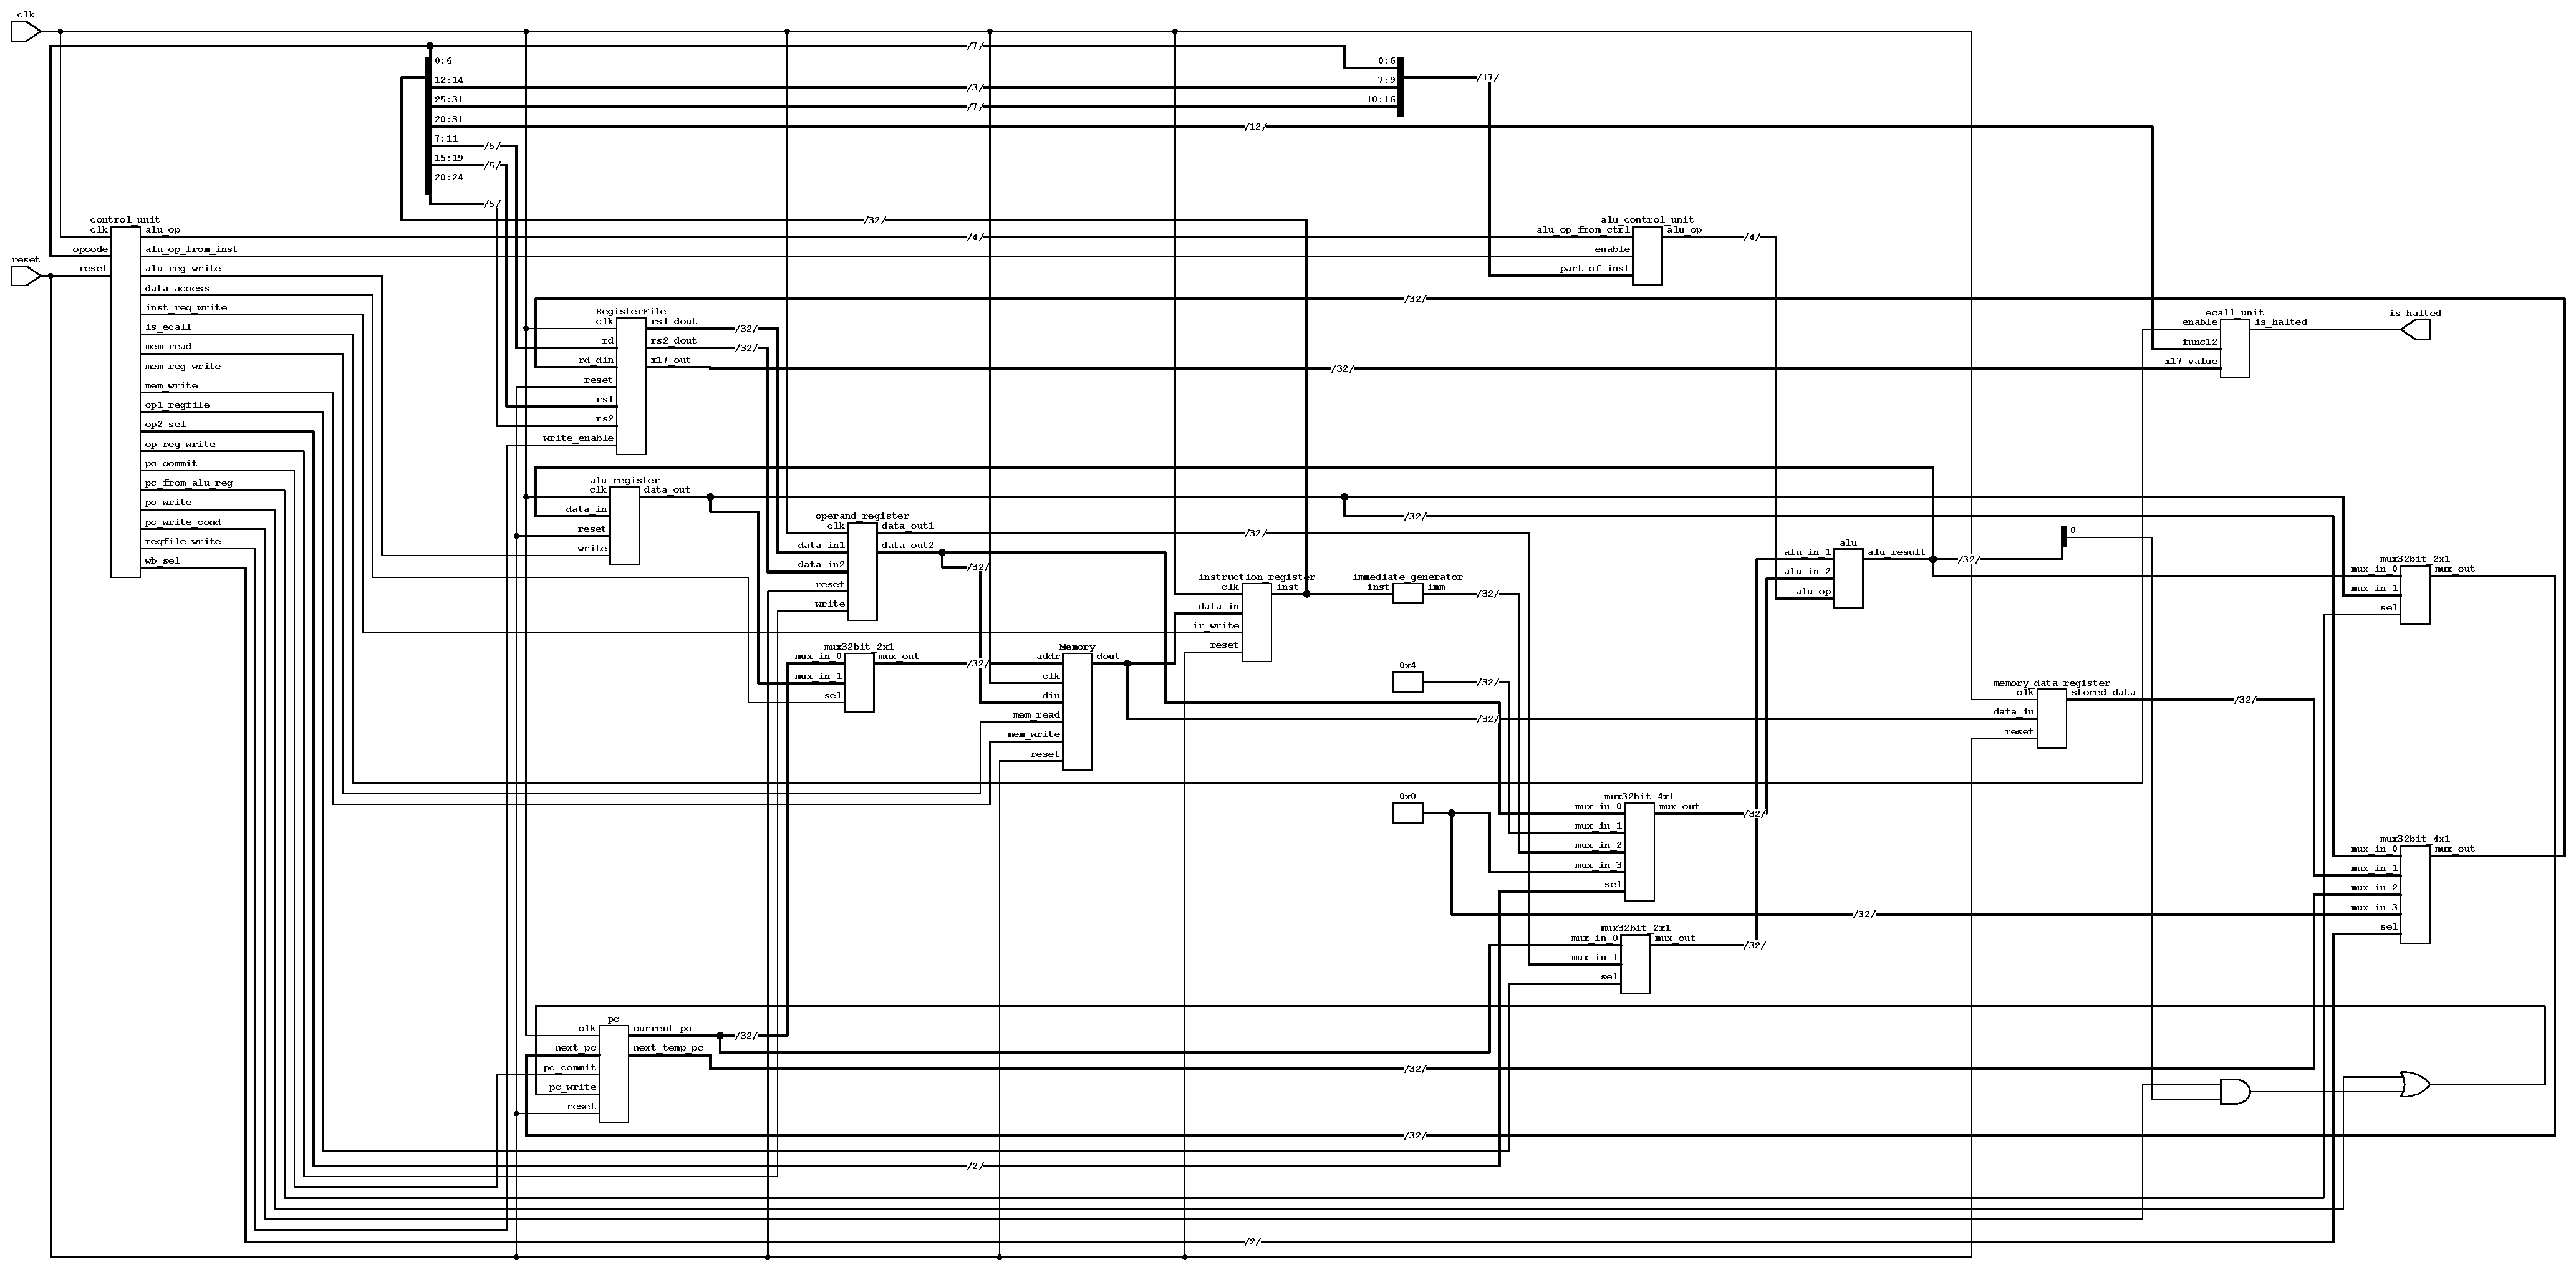
\includegraphics[angle=90,scale=0.35]{schematic.pdf}

\section{Discussion}

\subsection{Single-cycle CPU vs. Multi-cycle CPU}
Multicycle CPU와 Singlecycle CPU의 차이는 다음과 같다.
\begin{itemize}
  \item Staged -- 각 Unit의 재사용을 염두에 두고 Instruction의 실행을 Stage별로 구분하며, 이를 통해 필요 없는 Stage를 건너뛰는 방식으로 낭비되는 Cycle을 줄일 수 있다.
  \item Control Unit -- Stage Transition을 Control Unit에서 관리하기 때문에, 각 Instruction별로 해당하는 Stage transition의 FSM 정보를 Control Unit이 저장하도록 구현된다.
  \item Resource reuse -- \texttt{PC + 4} 혹은 \texttt{PC + imm} 등을 위해 추가적으로 Adder를 구성하지 않고, Control signal으로 Stage를 구분하여 겹치는 Stage가 없도록 ALU를 재사용한다.
  Memory 또한 Instruction memory와 Data memory를 구분하지 않고, 하나의 Memory unit에서 각기 다른 address로의 접근을 Multiplexer를 사용해 Control하는 방식으로 구현된다.
\end{itemize}

\subsection{Instruction Count of testbenches}
Control Unit의 Instruction Fetch Stage에서 Instruction의 type을 \texttt{\$display}를 통해 출력하고,
Instruction의 개수를 세었다.
\begin{center}
  \begin{tabular}{ | c | c | c | c | c | c | c | c | }
    \hline
    \textbf{Testbench} & \textbf{Arith.} & \textbf{Arith. Imm.} & \textbf{Load} & \textbf{Store} & \textbf{Branch} & \textbf{\texttt{JAL}} & \textbf{\texttt{JALR}}\\ \hline
    \texttt{basic\_mem} & 5 & 11 & 6 & 5 & 0 & 0 & 0 \\ \hline
    \texttt{ifelse\_mem} & 0 & 14 & 9 & 6 & 4 & 0 & 0 \\ \hline
    \texttt{loop\_mem} & 20 & 37 & 95 & 45 & 22 & 2 & 0 \\ \hline
    \texttt{non-controlflow\_mem} & 11 & 18 & 4 & 4 & 0 & 0 & 0 \\ \hline
    \texttt{recursive\_mem} & 23 & 332 & 228 & 168 & 41 & 62 & 41 \\
    \hline
  \end{tabular}
\end{center}
앞서 서술한 장점 중 Microsequence를 통해 Clock cycle을 줄일 수 있다는 점이 Multicycle CPU의 장점이다.
현 Multicycle CPU의 구현에서 사용하는 Cycle 개수는 다음과 같다.
\begin{itemize}
  \item Load -- 5 Cycle
  \item Arith., Arith. Imm., Store -- 4 Cycle
  \item Branch, \texttt{JAL}, \texttt{JALR} -- 3 Cycle
\end{itemize}
Single Cycle CPU에서는 Instruction 종류에 관계 없이, Instruction Fetch부터 Write Back까지의 5 Cycle을 요하게 된다.
각 Instruction별 Cycle 수를 곱하여 Speedup을 비교해보면 다음과 같다.
\begin{center}
  \begin{tabular}{ | c | c | c | c |}
    \hline
    \textbf{Testbench} & \textbf{Single-cycle CPU} & \textbf{Multi-cycle CPU} & \textbf{Speedup}\\ \hline
    \texttt{basic\_mem} & 135 & 114 & 1.184 \\ \hline
    \texttt{ifelse\_mem} & 165 & 137 & 1.204 \\ \hline
    \texttt{loop\_mem} & 1105 & 955 & 1.157 \\ \hline
    \texttt{non-controlflow\_mem} & 185 & 152 & 1.217 \\ \hline
    \texttt{recursive\_mem} & 4475 & 3664 & 1.221 \\
    \hline
  \end{tabular}
\end{center}
최대 약 1.2배의 Speedup을 확인할 수 있었다.


\section{Conclusion}
주어진 testbench 파일들이 테스트를 통과함을 확인할 수 있었다.

\texttt{basic\_mem.txt}에 대한 실행 결과는 다음과 같다.

\begin{lstlisting}
  ### SIMULATING ###
  TEST END
  SIM TIME : 234
  TOTAL CYCLE : 116 (Answer : 116)
  FINAL REGISTER OUTPUT
  0 00000000
  1 00000000
  2 00002ffc
  3 00000000
  4 00000000
  5 00000000
  6 00000000
  7 00000000
  8 00000000
  9 00000000
  10 00000013
  11 00000003
  12 ffffffd7
  13 00000037
  14 00000013
  15 00000026
  16 0000001e
  17 0000000a
  18 00000000
  19 00000000
  20 00000000
  21 00000000
  22 00000000
  23 00000000
  24 00000000
  25 00000000
  26 00000000
  27 00000000
  28 00000000
  29 00000000
  30 00000000
  31 00000000
  Correct output : 32/32
\end{lstlisting}

\texttt{ifelse\_mem.txt}에 대한 실행 결과는 다음과 같다.

\begin{lstlisting}
  ### SIMULATING ###
  TEST END
  SIM TIME : 280
  TOTAL CYCLE : 139 (Answer : 139)
  FINAL REGISTER OUTPUT
   0 00000000
   1 00000000
   2 00002ffc
   3 00000000
   4 00000000
   5 00000000
   6 00000000
   7 00000000
   8 00000000
   9 00000000
  10 00000000
  11 00000000
  12 00000000
  13 00000000
  14 0000000a
  15 00000028
  16 00000000
  17 0000000a
  18 00000000
  19 00000000
  20 00000000
  21 00000000
  22 00000000
  23 00000000
  24 00000000
  25 00000000
  26 00000000
  27 00000000
  28 00000000
  29 00000000
  30 00000000
  31 00000000
  Correct output : 32/32
\end{lstlisting}

\texttt{loop\_mem.txt}에 대한 실행 결과는 다음과 같다.

\begin{lstlisting}
  ### SIMULATING ###
  TEST END
  SIM TIME : 1916
  TOTAL CYCLE : 957 (Answer : 977)
  FINAL REGISTER OUTPUT
  0 00000000
  1 00000000
  2 00002ffc
  3 00000000
  4 00000000
  5 00000000
  6 00000000
  7 00000000
  8 00000000
  9 00000000
  10 00000000
  11 00000000
  12 00000000
  13 00000000
  14 0000000a
  15 00000009
  16 0000005a
  17 0000000a
  18 00000000
  19 00000000
  20 00000000
  21 00000000
  22 00000000
  23 00000000
  24 00000000
  25 00000000
  26 00000000
  27 00000000
  28 00000000
  29 00000000
  30 00000000
  31 00000000
  Correct output : 32/32
\end{lstlisting}

\texttt{non-controlflow\_mem.txt}에 대한 실행 결과는 다음과 같다.

\begin{lstlisting}
  ### SIMULATING ###
  TEST END
  SIM TIME : 316
  TOTAL CYCLE : 157 (Answer : 157)
  FINAL REGISTER OUTPUT
  0 00000000
  1 00000000
  2 00002ffc
  3 00000000
  4 00000000
  5 00000000
  6 00000000
  7 00000000
  8 00000000
  9 00000000
  10 0000000a
  11 0000003f
  12 fffffff1
  13 0000002f
  14 0000000e
  15 00000021
  16 0000000a
  17 0000000a
  18 00000000
  19 00000000
  20 00000000
  21 00000000
  22 00000000
  23 00000000
  24 00000000
  25 00000000
  26 00000000
  27 00000000
  28 00000000
  29 00000000
  30 00000000
  31 00000000
  Correct output : 32/32
\end{lstlisting}

\texttt{recursive\_mem.txt}에 대한 실행 결과는 다음과 같다.

\begin{lstlisting}
  ### SIMULATING ###
  TEST END
  SIM TIME : 7334
  TOTAL CYCLE : 3666 (Answer : 3686)
  FINAL REGISTER OUTPUT
  0 00000000
  1 00000000
  2 00002ffc
  3 00000000
  4 00000000
  5 00000000
  6 00000000
  7 00000000
  8 00000000
  9 00000000
  10 0000000d
  11 00000000
  12 00000000
  13 00000000
  14 00000001
  15 0000000d
  16 00000015
  17 0000000a
  18 00000000
  19 00000000
  20 00000000
  21 00000022
  22 00000000
  23 00000037
  24 00000059
  25 00000000
  26 00000000
  27 00000000
  28 00000000
  29 00000000
  30 00000000
  31 00000000
  Correct output : 32/32
\end{lstlisting}

\pagebreak

\section{Appendix -- Control Unit Code}
Evaluation Criteria에서 요구한 Control Unit Code의 스크린샷을 분할하여 첨부했다.
(22page 좌) - (22page 우) - (23page) 순서로 \texttt{control\_unit.v}를 구성한다.

\begin{center}
  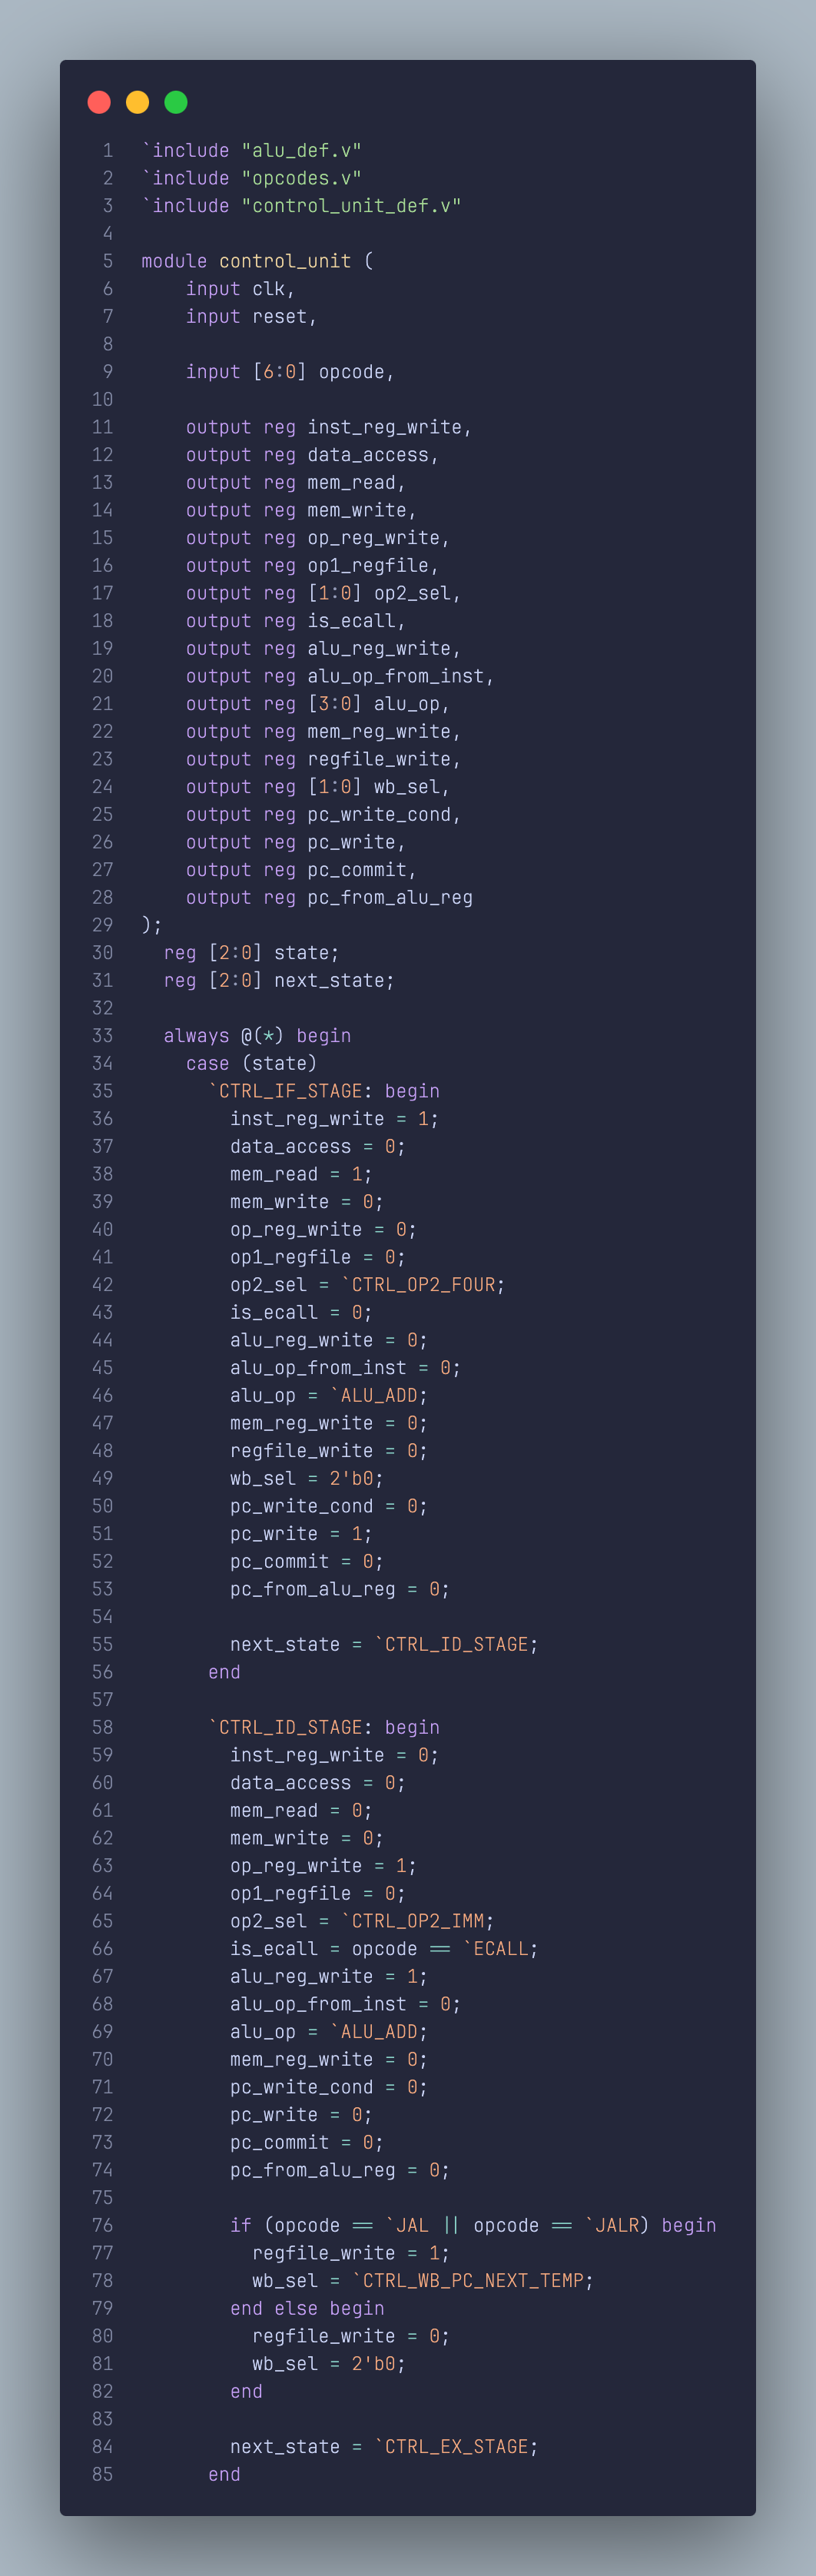
\includegraphics[scale=0.15]{code_screenshot/control_unit_1.png}
  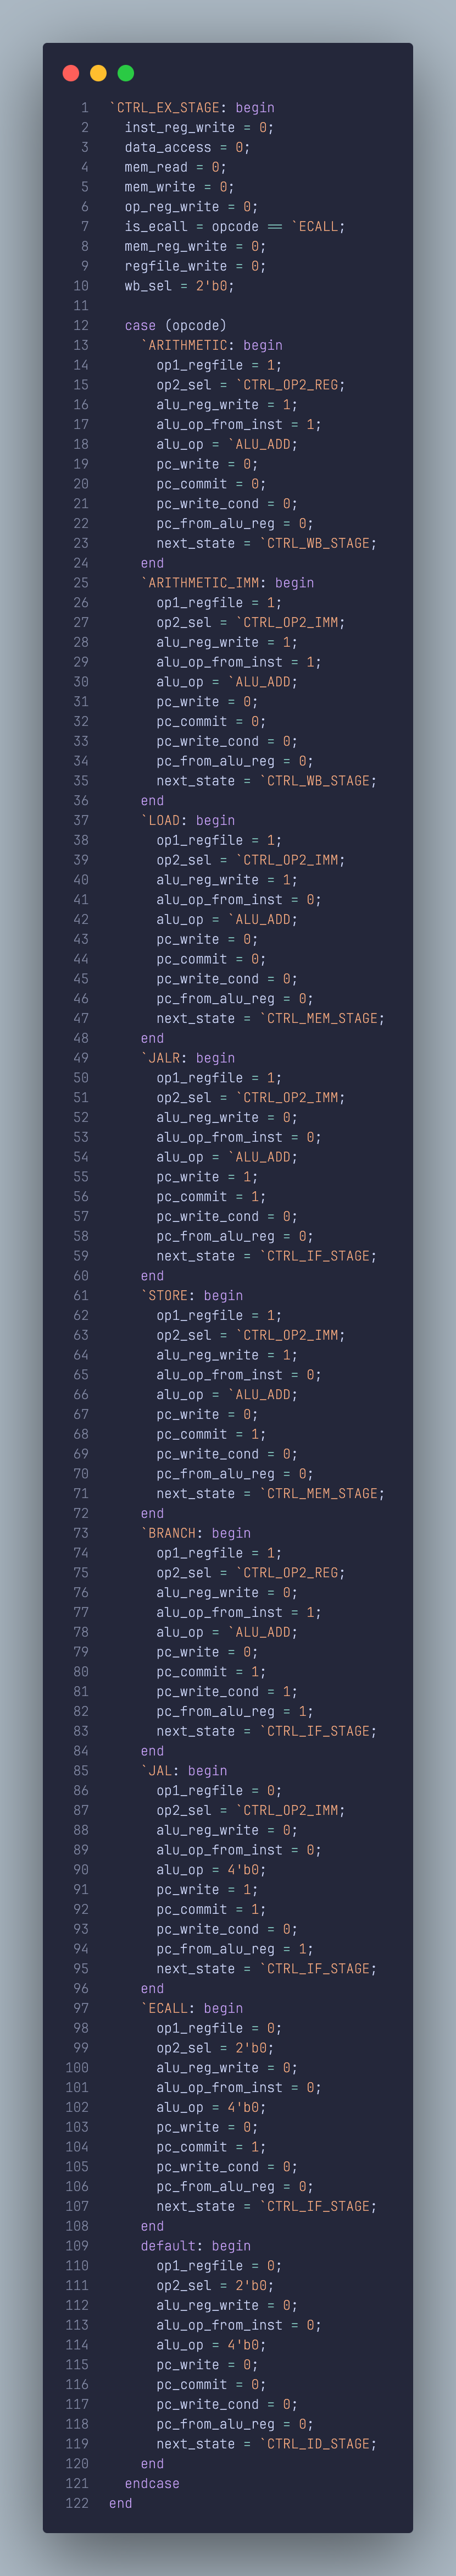
\includegraphics[scale=0.15]{code_screenshot/control_unit_2.png}
  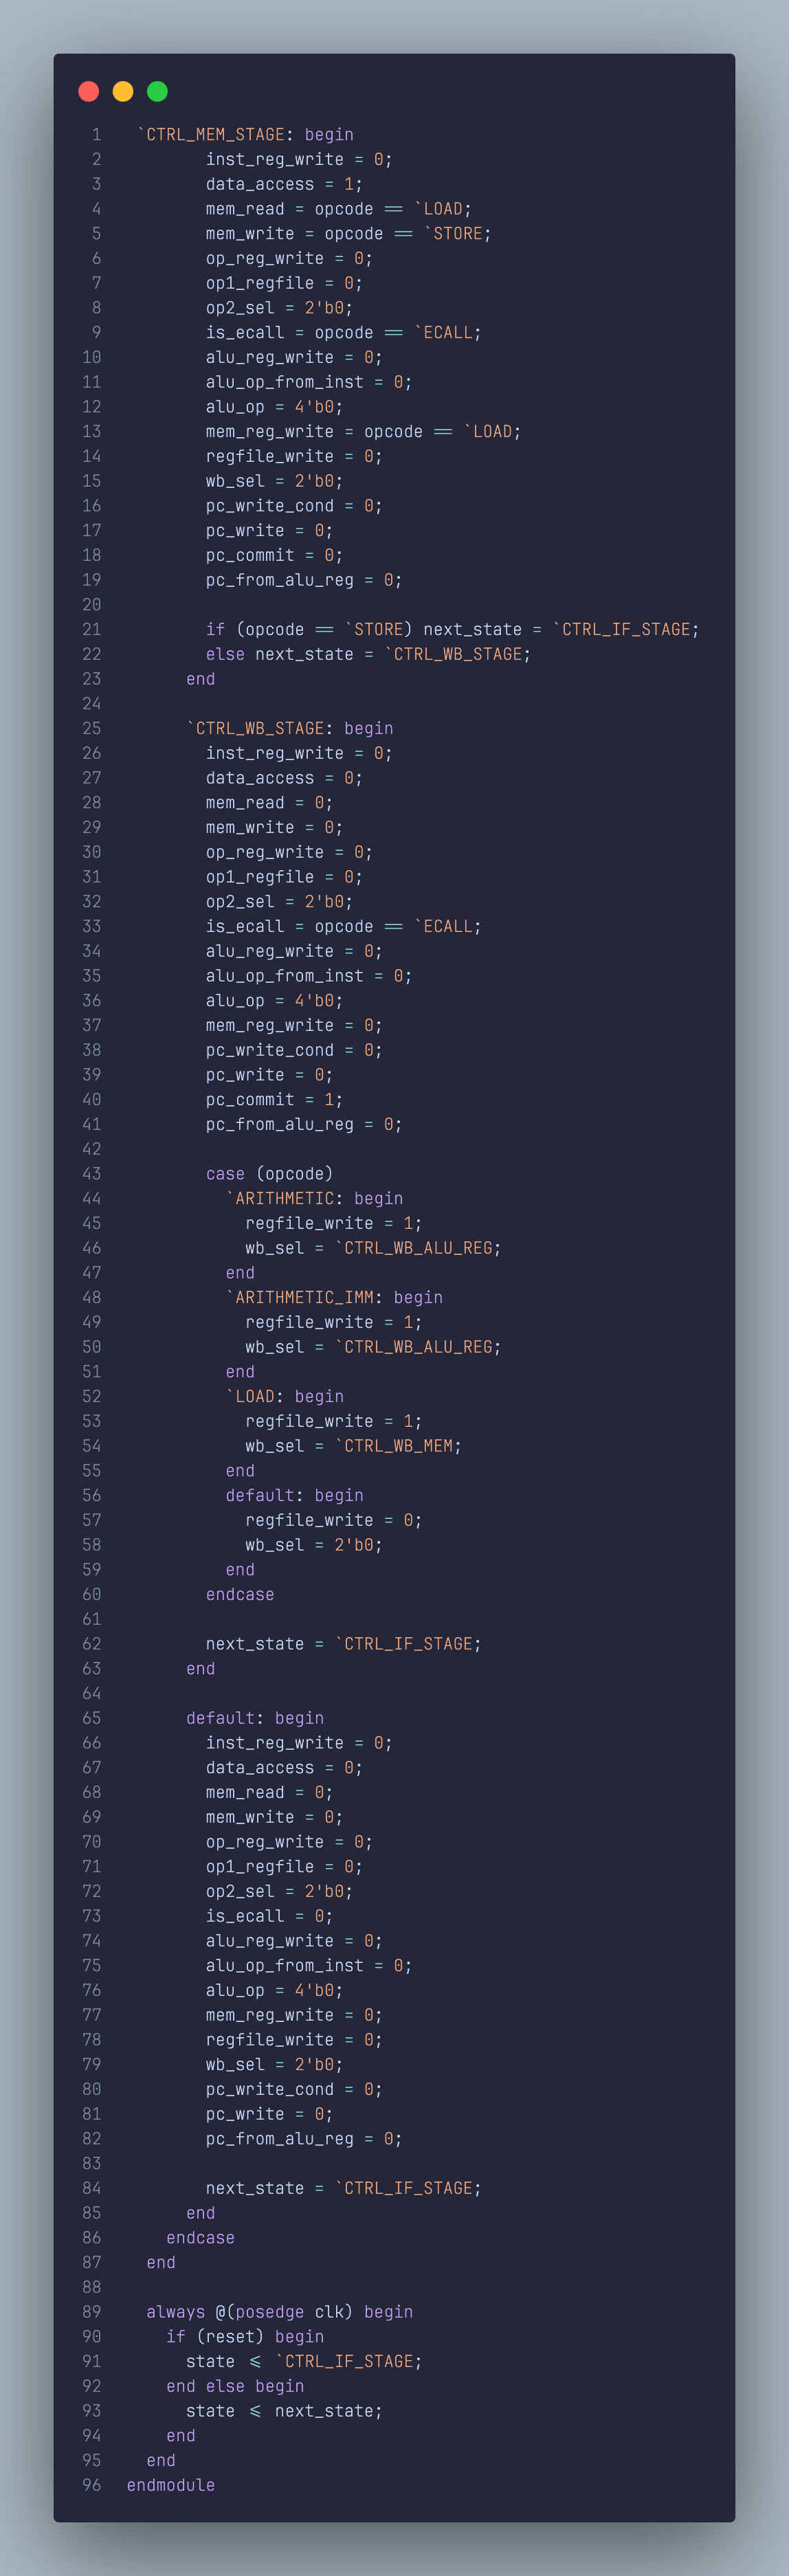
\includegraphics[scale=0.15]{code_screenshot/control_unit_3.png}
\end{center}

\end{document}
% vim: textwidth=79
